\documentclass[a4paper,12pt]{article}



\usepackage[parfill]{parskip}
\usepackage{graphicx}
\usepackage{booktabs}
\usepackage{listings}
\lstset{
    escapeinside={(*}{*)}
}
\usepackage{multirow}

\title{AutoRSpec}
\date{2017-04-25}
\author{Dan Shreeve}

\begin{document}

\pagenumbering{roman}
\addcontentsline{toc}{section}{Title page}
\maketitle

\newpage
\addcontentsline{toc}{section}{Signed declaration}
\section*{Signed declaration}
All sentences or passages quoted in this report from other people's work have been specifically acknowledged by clear cross-referencing to author, work and page(s). Any illustrations which are not the work of the author of this report have been used with the explicit permission of the originator and are specifically acknowledged. I understand that failure to do this amounts to plagiarism and will be considered grounds for failure in this project and the degree examination as a whole.
\par Name: Daniel Demaine Shreeve
\par Signature: .................................
\par Date: 03/05/2017

\newpage
\addcontentsline{toc}{section}{Abstract}
\begin{abstract}
Software Testing benefits the development and maintenance of a system by increasing quality and reliability. Software Testing also contributes around half of the cost of producing a system. Automating part or whole of this process reduces the cost while maintaining the benefits. The aim of this project is to produce a system that automatically generates RSpec test cases for model validation in Ruby on Rails. The tests will be generated from a formal database specification that the user has defined using the system. A file can be generated and inserted into the users application and run as though they been written by the user. The time taken to insert the information should be less than the time taken to write the tests manually, otherwise the user does not benefit.
\end{abstract}

\newpage
\addcontentsline{toc}{section}{Acknowledgements}
\section*{Acknowledgements}
First and foremost I would like to thank my supervisor \textbf{Dr. Gordon Fraser} for accepting my proposed project and providing impeccable advice and guidance throughout the process.
\par Finally I would like to thank my parents, \textbf{Linda Shreeve} and \textbf{Paul Shreeve}, and my grandparents \textbf{Elsie Marsden} and \textbf{Ray Marsden} for giving me the oppurtunity to go to university and supporting me throughout.

\newpage
\tableofcontents

\newpage	
\pagenumbering{arabic}
\section{Chapter 1: Introduction}
\par How severe can the consequences be from an error in a piece of software? In 1983 a bug in a piece of software nearly started World War Three.
\vspace{5mm}
\par During the Cold War, tensions between the US and Soviet Russia were extremely high. A Soviet early warning system had detected the launch of five ballistic missiles from the US. The only reason that Soviet Russia did not retaliate, starting World War Three, was the fact that Lt Col Stanislav Petrov had a "...funny feeling in my gut"\cite{ZDNetDisasters} and concluded that if the US was launching a full scale attack they would launch more than five missiles. The error in the system was discovered to be a bug in part of the software that distinguished false missiles from satellites picking up the reflection of sunlight from the top of clouds.\cite{ZDNetDisasters} If the bug in the code has falsey detected more missiles the world could be a very differn't place today.
\vspace{5mm}
\par Software testing increases the relability of a system and quality, by detecting errors and bugs which can be fixed, quality can aslo be further improved by tests proving it meets its design requirements. Software testing however is very costly, accounting for half the time put into development of a system and half of total expenditure.\cite{myers2011art} Automating part or the whole of the software testing process reduces the costs of testing while maintaining its benefits.
\vspace{5mm}
\par The motivation for this project is to bring the benefits of automated testing to Ruby on Rails. Ruby on Rails is a web application framework that allows developers to create fully functioning applications in a short of space of time. The reduction in time spent implementing increases the proportion of time spent testing. Thefore Ruby on Rails would benefit greatly from automated testing and also further encompass its time saving aspect.
\vspace{5mm}
\par The project aims to create a system that Ruby on Rails developers can use to reduce the development time of their projects by automatically generating all or part of the tests they require. The tests generated should not reduce the reliability and quality that manual written tests create.

\par WHATS TO FOLLOW GENERAL

\par WHAT CHP 2 IS ABOUT
\par WHAT CHP 3 IS ABOUT
\par WHAT CHP 4 IS ABOUT
\par WHAT CHP 5 IS ABOUT
\par WHAT CHP 6 IS ABOUT
\par WHAT CHP 7 IS ABOUT





\newpage
\section{Chapter 2: Literature Review and Research}




\subsection{Testing and Automation}
\par The European Space Agency spent ten years and \$7 billion designing and constructing the Ariane 5, a rocket that can launch multiple satellites into orbit from a single launch. Thirty nine seconds into its maiden voyage it exploded, destroying the Ariane 5 and its contents of four uninsured, extremley expensive scientific satellites. The explosion was caused by its own self-destruct sequence which was triggered automatically as the boosters were being torn away by aerodynamic forces. The extreme aerodynamic forces were caused by the rocket trying to recorrect its course due to flight data provided the guidance system. The guidance system had crashed and shutdown, along with its backup, the flight data provided that caused the rocket to readjust its course was actually a diagnostic error message. 
\vspace{5mm}
\par The cause of the shutdown was the guidance system trying to convert the sideways velocity of the rocket from 64-bit to 16-bit where an overflow occured causing the system to shutdown. To make matters worse, the programmers were aware that it could overflow but assumed that particular variable would never be large enough as it was used to prepare for launch and not in flight. However it was decided the system should run into the first forty seconds of flight, incase of a brief hold in the launch countdown, to make restarting the system easier. A known flaw in a system, that could of been handled, ended up causing the chain of events that led to the rocket exploding\cite{Ariane5}.
\vspace{5mm}
\par Software disasters can be caused by poor testing practices\cite{mcquaid2012software}, if the correct testing procedures and practices were in place in the previous example and the Soviet Guidance System example from the Introduction these situations could of been avoided. Software testing is therefore extremely important and should be included in the development of all applications. What is software testing and how does it help avoid these situations ?
\vspace{5mm}
\par Software testing is an investigation into a piece of software that provides information during development and maintenance. A process or series of process's are carried out that are designed to make sure computer code does what it designed to do and is absent of unintended behaviour\cite{myers2011art}. The information retrived from the proccess's can be used to track the progress during development against acceptance criteria and detect and locate errors and bugs. Errors and bugs detected within the code of the are immediatley known and can be handled, providing a smoother and more consistent development and maintenance flow. Software testing provides a more reliable and higher quality product when used as part of the development process due to these benefits.
\vspace{5mm}
\par Testing however can not guarantee that a program or peice of code is without errors, therefor completing testing is impossible. This is why the design of tests is vital to the integrity of the testing, making the tests as complete as possible. Given the constraints on time and cost, effective testing is simply "What subset of all possible test cases has the highest probability of detecting the most errors?"\cite{myers2011art}. Tests are designed using information about the program along with its intended behaviour. In a given environment, with proper determined input, there is an expected behaviour/output. If the code undertest does not display the desired outcome it is said to of failed the test. 
\vspace{5mm}
\par A 'test case' will test a very specific behaviour of a program. A collection of test cases is a 'test suite', representing that a certain section of the system has a specificied set of behavoiurs. A relevant example would be for a table in a database. The test suite would represent if the table has the desired validations in place and would consist of test cases that tested each specific behaviour in isolation. The tests would be run as a set to confirm the table has the desired behaviour, while being in the case of undesired behaviour being to specify which test case, therefore highlight the exact error in the code. Design of test cases is important and to design a test information is required, the information is sourced in two main ways Functional and Structural.
\vspace{5mm}
\par  Functional Testing also known Black-box testing, is the technique of creating test cases with information from a formal or informal functional specification. A functional specification is the description of intented program behaviour distinct from the program itself. The software requirements and or its design specification are most commonly used to derive the functional specification. The software entity under test is treated as a black box, the actual code implementation is not known, where proper inputs are fed in and the output is observed. If the output or behavior is that specified in the specification the test has passed otherwise it has failed. Example: When a user clicks the Home tab in the nav bar they are directed to the Home page, in this case the input is the user clicking the home tab and the desired behaviour is being directed to the home page. Black box testing can detect some faults that white box cannot, such as absent behaviours that are in the requirements but not coded in as they were missed. The systematic nature can help avoid missed test cases and provide more consistent coverage.\cite{nidhra2012blackbox}\cite{young2008software}
\vspace{5mm}
\par One approach to functional testing is a systematic approach. A systematic approach has four steps :\cite{young2008software}
\vspace{5mm}
\begin{enumerate}
\item Partition the functional specification into independently testable features using a divide and conquer approach. For a database table, dividing a table in a databse into its fields, then dividing again into each fields properties. 
\item For each independently testable feature find a representative class of values or derive a model to test it. For a string field with property of length greater than five. We may derive a specail case of blank string, a string of length less than five and string with length greater than five
\item Generate test case specifications. Finding concrete values for the reprensentive class of values or model above. Building on the previous example we may have \{ "", "less" ,"longer"\}
\item Generate test cases and instantiate tests, turning specifactions into tests and instantiating them.
\end{enumerate}
\vspace{5mm}
\par Structural testing, also known as White box testing. uses the physical implementation of the software itself such as source code as information to produce test cases. A common approach to white box testing is 'Control Flow' testing. Due to the nature of code varying greatly between projects and the complexity and detail that can be involved the following steps are greatly simplified while maintaining the core principle.
\vspace{5mm}
\begin{enumerate}
\item Identify a feature to be tested. This could be on a small or large scale, for our examples we will choose creating an entry on a database.
\item Create a flow graph plotting all steps and paths the feature can execute, this would include steps such as verification.
\item Identify paths through the flow graph, entry is created successfully and displayed or unsuccessfuly and prompted with an error message.
\item For each path write a test case that is expected to execute this path, with valid variables an entery should be created and it should be displayed.
\end{enumerate}
\vspace{5mm}
\par Software testing is necessary and very costly. "In a typical programming project approximately 50 percent of the elapsed time and more than 50 percent of the total cost were expended in testing the program or system being developed"\cite{myers2011art}. Reducing the costs, both time and monetary, is the main motivation for Automated Testing. Another overlooked and unappreciated benefit of automating testing is test case generation is one the most intellectully demanding and critical challenges in software testing.\cite{anand2013orchestrated} By automating this process it not only reduces costs but also allows developers to dedicate more time and effort to other areas, also in some cases it is harder to create a test case but easy to verify a generated test case is correct. A whole systems tests do not have to be automatically generated to reduce costs and benefit.
\vspace{5mm}
\par An Automated functional testing approach follows the same methodology as manual systematic generation of test cases. Each step is automated and follows the same principles. The information as before used to derive test cases is the functional specification. The functional specification is however only formal  and has specified syntax so that it can be interpreted by the system that will generate the test cases. There is more creativitivy and design put into the functional specification as the test designer is usually limited to a choice of test selection criteria. For step 3 the system must also include value generation that can meet the representative class of values outlined in step 2.\cite{young2008software}
\vspace{5mm}
\par Automated functional testing tends to be more complex, as it has to understand and interpret human written code. One method that has recieved alot of attention from researchers and is similar to Control Flow is Symbollic Execution, where symbollic values are used to instead of concrete values for program inputs. Programs variables are described by the symbolic expressions of those inputs. The state of the program includes the symbolic values of program variables, a program counter and the path contraint on symbolic values: a boolean formula over the symbolic values input. Using this method it can explore all possible path divergences through a system and identify stop points, where the path ends. The major problem with automated white box testing is identifying if a behaviour, stop point or a specific divergence in Symbollic execution, is desired or not. This problem is known as the Oracle problem, as desired behavoiur of code is contained within its specfication and design, not its implementation. Therefore some level of user input is required.\cite{anand2013orchestrated}
\vspace{5mm}
\par Another relevant challenge Symbolic Execution is developing a system that developing system that can cover multiple languages at once is very complex and producing a system can produce feasible output can be impossible due to the path divergence problem, where either a user has to specify so many models it isn't automated wnough to benefit or it doesnt find a signifcant amount of feasible program paths. As Ruby on Rails design environment can vary drastically between projects due to the flexibility of its framwork and use of Gems I will only consider and that some level of User input is required I will only consider Black Box testing techniques when I come to designing the project. This will deliver a product that will be usable to a wider audience as it is dependent upon on specification for which I can define. Interpreting multiple languages and being flexible enough to be useful is out of the scope of this project.
\vspace{5mm}
\par PARAGRAPH SAYING BB CHOSEN SO VALUE GENERATION NEEDS TO BE CONSIDERED WHEN CHOOSING TOOLS

\subsection{Testing in Rails}

\par Ruby on Rails applications are primarily developed using the generation of skeletons with variables set by the developer. The skeletons save a vast amount of time by generating a default environment which can then be built upon according to the section under development. By default one of the files created is a test file and it uses the Ruby on Rails MiniTest class.\cite{railsTest}

\par TEST UNIT

\par RSPEC

\par CONCLUDE RSPEC

\par RSPEC IN GREATER DETAIL (may be few par)

\par TEMPLATES FOR RSPEC - NEED STRING MANIPULATION ETC

\par FACTORY GIRL



\subsection{Tools to use}
\par TOOL REQUIREMENTS FROM PREVISOUS SECTIONS
\vspace{5mm}
\par An MVC web application fits all these criteria. MVC, Model-View-Controller is an architectural pattern that seperates an application into three interconnected parts. The separation allows for responsibilities to be allocated independently to each component, seperating the logic from the user. The model is responsible for the data of the application and the rules and logic used to create and update the information. The view is responsible for displaying the data and possible interactions with the system to the user. The controller is responsible for controlling the flow of the system,  accepting user input and converting it into commands for the model and view.
\vspace{5mm}
\par An example of the components interacting would be creating an entry to a database. The view would be responsible for displaying the form in which to fill in. On submission the controller will process the information, ensure only persmissable information is submitted and enter additional information, then send it to the model. The model would verify the structure of the information, correct fields are present and cohere with its rules. The model will then notify the controller if the submission was successful or not and the controller will update the view to reflect the status.
\vspace{5mm}
\par The seperation means that all user interaction with the database has to go through the controller and is therfore limited to what the developers want users to be able to do. This provides a high level of security as each action is controlled and the internal structure and representation of the information within the database is hidden. Simultaneous development is also possible due to the seperation of the components, work on the front and back end concurrently. Although I will not be able to get the full benefit of this as I am developing the project solo, it will allow me to shift focus as components do not need to finished before switching to another, giving greater flexibility in development. 
\vspace{5mm}
\par High levels of cohesion are inherited automatically from the architecture with the grouping of logically similar elements, this makes the code easier to read and creates a more natural flow within the source code. There are however some drawbacks to MVC architecture, they are inheritly more complex due to the seperation and the framework must be learnt in addition to the programming language it is in, which there can be multiple languages between the components. This steep learning curve could mean a large initail investment into a team learning a new framework along with its languages.
\vspace{5mm}
\par MVC web application frameworks have become extremely popular and are behind some of the most used and powerful websites. Django an MTV, follows MVC architecture but its creators decided to rename the components \cite{Django} to better suit them, is behind the two most visted websites in the world Google and YouTube\cite{SHUUP}\cite{Alexa}. Ruby on Rails another MVC is behind Twitter, Airbnb and Soundcloud.\cite{Coderfactory} MVC frameworks are known for their scalablity, being suitable for the smallest to the largest projects. However FaceBook decided that its scalablity had reached its limit, that adding new features made the code exponentailly more complex.\cite{Infoq} My project will be no where near the scale of facebooks sourcecode so I do not need to worry about reaching the end of its scalibilty.
\vspace{5mm}
\par The chosen MVC to construct the project in is Ruby on Rails. I have done previous projects in both Ruby and the Rails framework, the rest of this section will show that Ruby on Rails is an adequate choice.
\vspace{5mm}
\par Ruby was selected as the primary programming language by default as it is the language that runs Ruby On Rails. Ruby is a dynamic, multi-paradigm programming language. The paradigms consist of Object-oriented, Imperative, Functional and Reflective making it a very powerful and versatile language. This combination is from its founder ‘Yukihiro Matsumoto’ who was influenced by Perl, Smalltalk, Eiffel, Ada, and Lisp.
\vspace{5mm}
\par Ruby’s primary design goal was to “make a language that he himself enjoyed using, by minimizing programmer work and possible confusion”(Ruby Wiki). Achieved with a focus on human interaction, how programmers code and design applications as opposed to focusing on how the code will run on machines. And also following the principle of least astonishment, where the behaviour of the language minimizes confusion for experienced users.
\vspace{5mm}
\begin{figure}
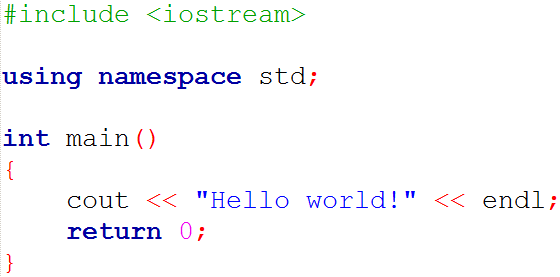
\includegraphics[width=\linewidth]{screenshots/c++_hello_world}
\caption{C++ print Hello world to console}
\label{fig:c++print}
\end{figure}
\begin{figure}
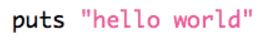
\includegraphics[width=\linewidth]{screenshots/ruby_hello_world}
\caption{Ruby print Hello world to console}
\label{fig:rubyprint}
\end{figure}
\par The above two images show C++ \ref{fig:c++print} and Ruby \ref{fig:rubyprint} printing ‘Hello world’ to the console. The comparison between the two languages highlights the efficiency and simplicity of the Ruby language.Ruby on Rails projects are commonly worked on by a group of people and in multiple languages, therefore the simplistic syntax gives greater clarity and understandability to programmers who are lesser experienced in Ruby.\cite{AboutRuby}
\par Ruby is open source, free and redistributable with a vast range of existing code from both Ruby and its large community. Primarily consisting of Gems, code packages that can be installed and supported into a project easily and with minimal effort via RubyGems, and frameworks, such as Ruby on Rails. Making it very popular for education and business. Following the DRY ‘Don't Repeat Yourself’ principle in a very effective and efficient manner.\cite{AboutRuby}
\par Ruby was ranked ninth on TIOBE index\cite{TOBIE} and has become a very popular and respected language relative to its age among the other languages on the index. No alternatives could be considered due to the dependency of Ruby on Rails on Ruby, however Ruby is a very strong and durable language so it does not detract from the overall project.
\vspace{5mm}
\par FORMS AND DATABASE SUPPORT FOR INPUTTING INFORMATION THAT CAN BE PROCESSED
\vspace{5mm}
\par STRING MANIPULATION FOR TEMPLATES
\vspace{5mm}
\par NUMBER GENERATION
\vspace{5mm}
\par STRING GENERATION FROM REGEXP USING GEM REGEXP.RANDOM
\vspace{5mm}
\par RUBY HAS NECESSARY LOGIC TO CONTROL FLOW ETC


\subsection{Evaluation}
\par HOW TESTS ARE EVALUATED
\par HOW OTHER PEOPLE EVALUATED PROJECTS
\par INJECTION
\par DOG FEED
\par COMPARE OUTPUT WITH WHAT EXISTING HAD
\par COMPARE CODE COVERAGE
\par TIME SAVED


\newpage
\section{Chapter 3: Requirements and Analysis}
\par REFINE AIM INLINE WITH LIT REVIEW TO "TO PROVIDE A SYSTEM THAT AUTOMATICALLY GENERATES MODEL TESTS IN RSPEC"
\par This project started with the motivation of bringing automated testing to Ruby on Rails. From research carried out and disscussed in Chapter 2 and considering the scale of the project the way to achieve this was to focus on validation in the model component and produce RSpec test cases. A more precise description of the project is therefore \textbf{To create a system that automatically generate RSpec test cases for model validation in Ruby on Rails Applications}. To accomplish this aim three main aspects of the system are as follows:

\begin{enumerate}
\item Allow a user to create and maintain a formal specifcation
\par A user should be able to describe all tables, fields and corresponding validation properties using the system. The user should also be able to edit and update the formal specification due to their changing demands.
\item Generate a valid RSpec test case
\par The RSpec test case should be generated with information entered from defined formal specification. To be valid the RSpec test case must meet certain critera. The test case must run the same as a manually produced user test case. It must only test the specified behaviour, e.g Employee table, Age field, must be greater than 18, and nothing else. It must produce a human readable test case with a human readable  behaviour descriptor that makes the user aware of exactly what behaviour has failed. It must produce a generated value that isolates the behaviour under test, it generates a value that fails the validation under test while passing the other validations for the field.
\item Consolidate all RSpec test cases for to make a valid test suite for a table
\par All test cases for a table, for all its fields and assigned validations, must be consolidated into a test suite that runs as a manual written test suite.
\end{enumerate}

\par To make the system viable and useful to developers there are some additional considerations
\begin{enumerate}
\item Ease of use
\par The system built should be easy and intuitive to use. 
\item Time saving
\item Creating the formal specification must take less time than it takes to write the tests manually
\end{enumerate}

\par Ruby on Rails has fourteen data types supported natively be ActiveRecord\cite{railsTableType}. Ruby on Rails also has many active record validations supported natively. To fit the scope of the project not all data types and validations will be supported. The selection of data types and validations supported are as follows.

\par Data Types Supported
\begin{enumerate}
\item Integer
\item Float
\item String
\end{enumerate}

\par Integer and Float Validations
\begin{enumerate}
\item Greater than
\item Greater than or Equal to
\item Equal to
\item Less than or Equal to
\item Less than
\item Other than
\item Divisible by
\item Blank
\item Inclusion
\item Exclusion
\end{enumerate}

\par String Validations
\begin{enumerate}
\item Maximum Length
\item Minimum Length
\item Exact Length
\item Format
\item Blank
\item Inclusion
\item Exclusion
\end{enumerate}


\begin{table}
\centering
\caption{Formal Specification Requirements}
\label{my-label}
\begin{tabular}{|l|l|l|}
\hline
\textbf{ID} & \textbf{Requirement}                                                   & \textbf{Priority} \\ \hline
\textbf{1}  & A user can create a Project                                            & \textbf{M}        \\ \hline
\textbf{2}  & A user can edit a Project                                              & \textbf{M}        \\ \hline
\textbf{3}  & A user can delete a Project, associated Tables are also deteled        & \textbf{M}        \\ \hline
\textbf{4}  & A user can create a Table, only for a given  Project                   & \textbf{M}        \\ \hline
\textbf{5}  & A user can edit a Table                                                & \textbf{M}        \\ \hline
\textbf{6}  & A user can delete a Table, associated Fields are also deteled          & \textbf{M}        \\ \hline
\textbf{7}  & A user can create a Field, only for a given Table                      & \textbf{M}        \\ \hline
\textbf{8}  & A user can edit a Field                                                & \textbf{M}        \\ \hline
\textbf{9}  & A user can delete a Field, associated validations are also deteled     & \textbf{M}        \\ \hline
\textbf{10} & A user can assign a validation and value, only for a given Field       & \textbf{M}        \\ \hline
\textbf{11} & A value must be valid for a validation to be assigned                  & \textbf{M}        \\ \hline
\textbf{12} & A user can edit a validation assignment and value                      & \textbf{M}        \\ \hline
\textbf{13} & A user can delete a validation assignment and value                    & \textbf{M}        \\ \hline
\textbf{14} & A user can view all Tables associated to a given Project               & \textbf{D}        \\ \hline
\textbf{15} & A user can view all Fields associated to a given Table                 & \textbf{D}        \\ \hline
\textbf{16} & A user can view all validations and values associated to a given field & \textbf{D}        \\ \hline
\end{tabular}
\end{table}

\begin{table}
\centering
\caption{RSpec Test Case Requirements}
\label{my-label}
\begin{tabular}{|l|l|l|}
\hline
\textbf{ID} & \textbf{Requirement}                                                                                                                       & \textbf{Priority} \\ \hline
\textbf{1}  & RSpec test case should be runnable                                                                                                         & \textbf{M}        \\ \hline
\textbf{2}  & RSpec test case should only test one behaviour                                                                                             & \textbf{M}        \\ \hline
\textbf{3}  & RSpec test case must should test behaviour intended                                                                                        & \textbf{M}        \\ \hline
\textbf{4}  & RSpec descriptor must be human readable                                                                                                    & \textbf{D}        \\ \hline
\textbf{5}  & When test case fails, its output must specify exact behaviour at fault                                                                     & \textbf{D}        \\ \hline
\textbf{6}  & RSpec test case should have human readable syntax                                                                                          & \textbf{D}        \\ \hline
\textbf{7}  & Be able to generate an Integer that satisfies all validations and their values assigned to a field                                         & \textbf{M}        \\ \hline
\textbf{8}  & Be able to generate an Integer that does not satisfy a validation but satisfies all other validations and their values assigned to a field & \textbf{M}        \\ \hline
\textbf{9}  & Be able to generate a Float that satisfies all validations and their values assigned to a field                                            & \textbf{M}        \\ \hline
\textbf{10} & Be able to generate a Float that does not satisfy a validation but satisfies all other validations and their values assigned to a field    & \textbf{M}        \\ \hline
\textbf{11} & Be able to generate a String that satisfies all validations and their values assigned to a field                                           & \textbf{M}        \\ \hline
\textbf{12} & Be able to generate a String that does not satisfy a validation but satisfies all other validations and their values assigned to a field   & \textbf{M}        \\ \hline
\end{tabular}
\end{table}

\begin{table}
\centering
\caption{RSpec Test Suite Requirements}
\label{my-label}
\begin{tabular}{|l|l|l|}
\hline
\textbf{ID} & \textbf{Requirement}                                          & \textbf{Priority} \\ \hline
\textbf{1}  & RSpec test suite should be runnable                           & \textbf{M}        \\ \hline
\textbf{2}  & RSpec test suite should be contain all test cases for a table & \textbf{M}        \\ \hline
\textbf{3}  & RSpec test cases should be grouped via field                  & \textbf{D}        \\ \hline
\textbf{4}  & RSpec test cases should be in a logical order                 & \textbf{D}        \\ \hline
\textbf{5}  & RSpec test suite must be available for download               & \textbf{M}        \\ \hline
\end{tabular}
\end{table}


\newpage
\section{Chapter 4: Design}

\subsection{Database}
\par The database was designed to accomodate the formal specification and extra information needed for RSpec test cases. Ruby on Rails has native support for relations via ActiveRecord, this provided flexability in being able to have many relations. The design paradigm of sole responsiblity was carried forward and each table has one purpose.

\begin{figure}
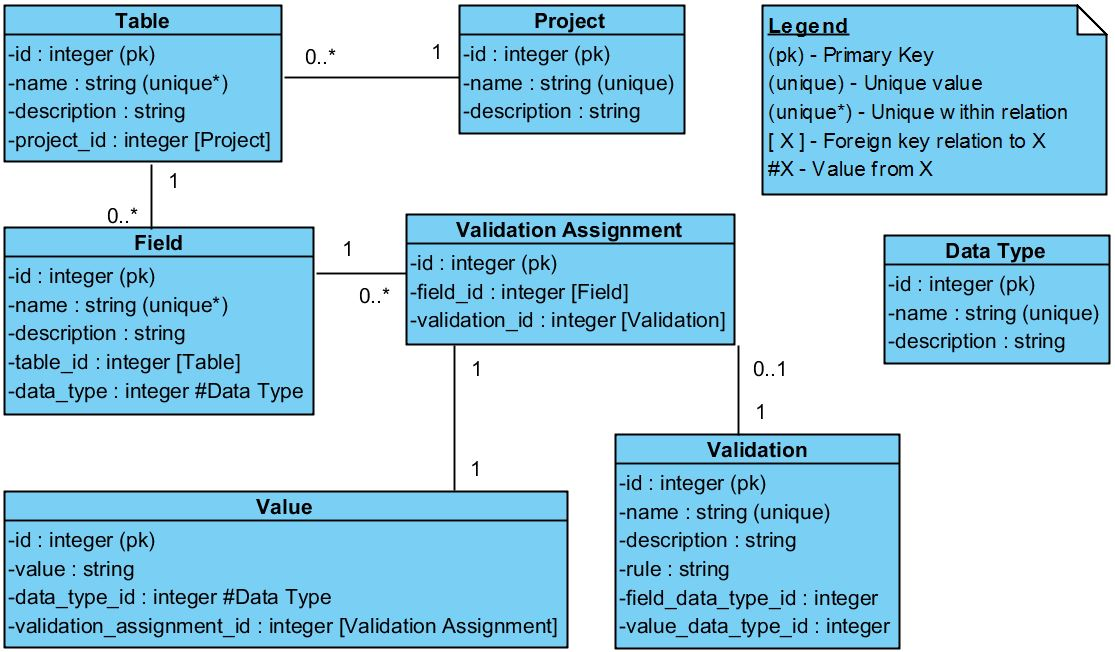
\includegraphics[width=\linewidth]{screenshots/databaseUML}
\caption{UML Database diagram}
\label{fig:UML1}
\end{figure}

\par \textbf{Project}
\par Project allows for a user to use the system for multiple projects, that is to organise groups of tables that are disconnected. The name field is unique to avoid confusion amongst projects. The description field is only for the user to add extra information if they desire and serves no functional purpose in the system. A project can have zero to many tables. When a project  is deleted its associated tables should also be deleted.

\par \textbf{Table}
\par Table is the table in a users database they are constructing a functional specification for. A table can only be created with a valid project\_id foreign key. The name is unique within the scope of the project, multiple tables can exist with the same name within the database but they must belong to seperate projects. The description field is only for the user to add extra information if they desire and serves no functional purpose in the system. A table belongs to a project and has zero to many fields. When a table is deleted its associated fields should also be deleted.

\par \textbf{Field}
\par Field is the field in a users database they are constructing a functional specification for. A field can only be created with a valid table\_id foreign key. The name is unique within the scope of the table, multiple fields can exist with the same name within the database but they must belong to seperate tables. The description field is only for the user to add extra information if they desire and serves no functional purpose in the system. Data\_type\_id is the fields data\_type and is limited to values in the Data Type table, however no relation is forced. A field belongs to a table and has zero to many Validations through Validation Assignments. When a table is deleted its associated validation assignments should also be deleted.

\par \textbf{Validation}
\par Validation is a validation the user can associate to a field. The user can not create, edit or destroy these and they are seeded in the database. The name is unique within the scope of its field\_data\_type. The description field is to aid the user is understanding what the validation is. The rule field is used within the system to generate values. Field\_data\_type\_id and value\_data\_type\_id limited to values in the Data Type table, however no relation is forced, and are used so only appropriate validations can be assigned to fields. A validation has zero to many fields through validation assignments.

\par \textbf{Value}
\par Value is the value of a validation that a user associates with a field, E.g false for blank or ten for minimum length. A value can only be creataed with a valid validation\_assignment\_id foreign key. The value is stored as a string and the data type of which the system should treat the value as is stored in data\_type\_id, which refers to the data type table, but no relation is enforced. A value belongs to a validation assignment.

\par \textbf{Validation Assignment}
\par Validation assignment associates a field with a validation and also the value for that validation. The assignment is created then a value is created belonging to the assignment. A validation assignment can only be created with both valid field\_id and validation\_id foreign keys. A validation assignment has one field, one validaiton and owns a value.

\par \textbf{Data Type}
\par Data type is used to provide consistency throoughout the system by checking data types are equal between entities, checking values of are the correct type and also used in forms to reduce options available to the user. The user can not create, edit or destroy these and they are seeded in the database. The name field is unique to avoid confusion amongst data types and avoid possible duplication. The description field is to clarify the user on the data type. Data  type has no relations, but is used throughout the system in reference.


\subsection{View and Flow}
\par Human centered design principles with the goal of increasing effectiveness, efficency and satisfaction\cite{maguire2001methods} were the main consideratons when designing the look and how the user navigates and uses the system.The principles taken into consideration and how they were applied are\cite{abras2004user}:

\begin{enumerate}
\item \textbf{Simplifying the structure of tasks}
\par An average user is able to remember five things at a time. Providing consistency within similar methods such as creations of entitys and also clearly displaying where in the system the user is reduces the strain on both long and short term memory. The creation, deletion and editing of entitys follows the familiar and consistent method of filling in a form and submitting it. At the top of each page it clearly displays how deep in the system and also the names of each level. This means the user will have to remember less when using the system.
\item \textbf{Exploiting the power of constraints}
\par Reducing and not exposing a user to redundant or irrelevant information allows a user to use a system more efficently and with less effort, by not having to process said information. This is used by displaying only the related entities when viewing an entity, only the fields for a table are shown when viewing that table. When a user is creating an entity with a form options are reduced to those that are valid, only choose from Integer validations for a Integer field. Entitys that are dependent on a another, field is dependent on table, are only available to create when viewing the dependent upon entity.
\item \textbf{Make things visible}
\par Bridging the gulf of execution, buttons and links do what a user expects them to do.  This principle followed by using standard naming conventions on standard objects such as buttons and links that a user is familiar with.
\end{enumerate}

\begin{figure}
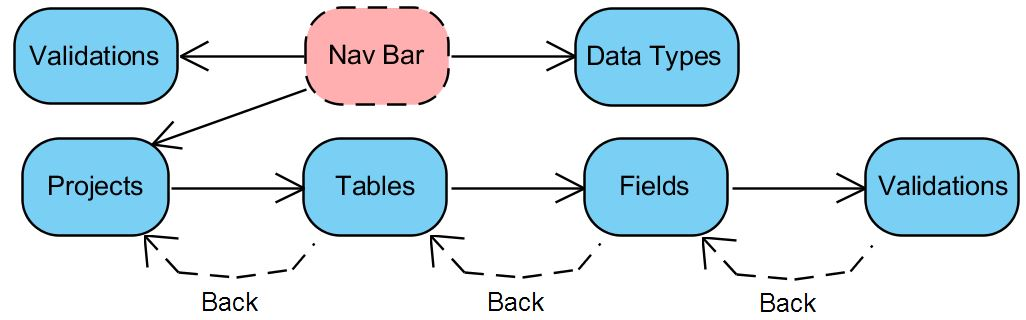
\includegraphics[width=\linewidth]{screenshots/pageflow}
\caption{The navigational flow of the system}
\label{fig:nflow}
\end{figure}


\begin{figure}
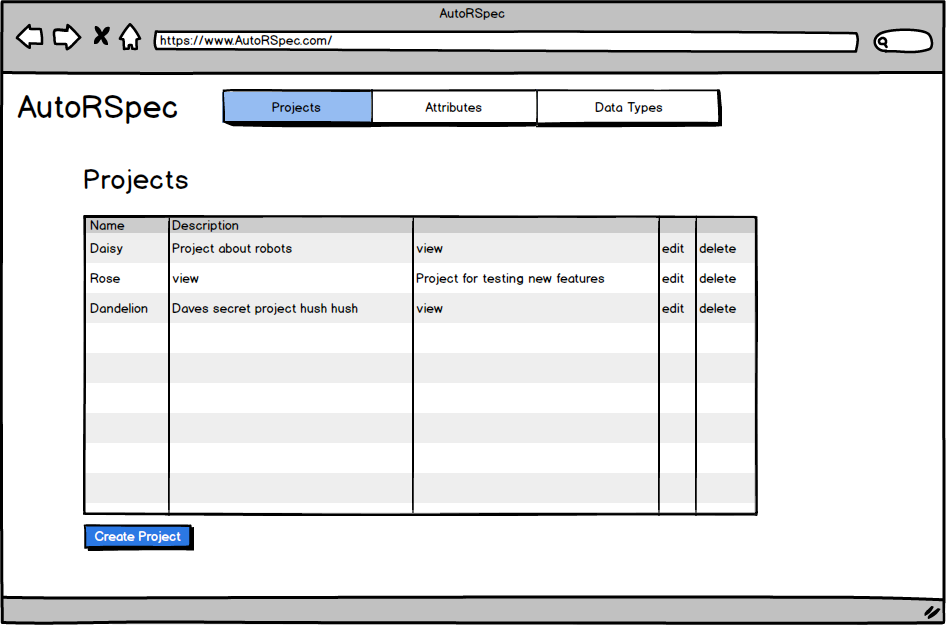
\includegraphics[width=\linewidth]{screenshots/muhome}
\caption{Mock up of projects page for the system, also home page. }
\label{fig:mu1}
\end{figure}

\begin{figure}
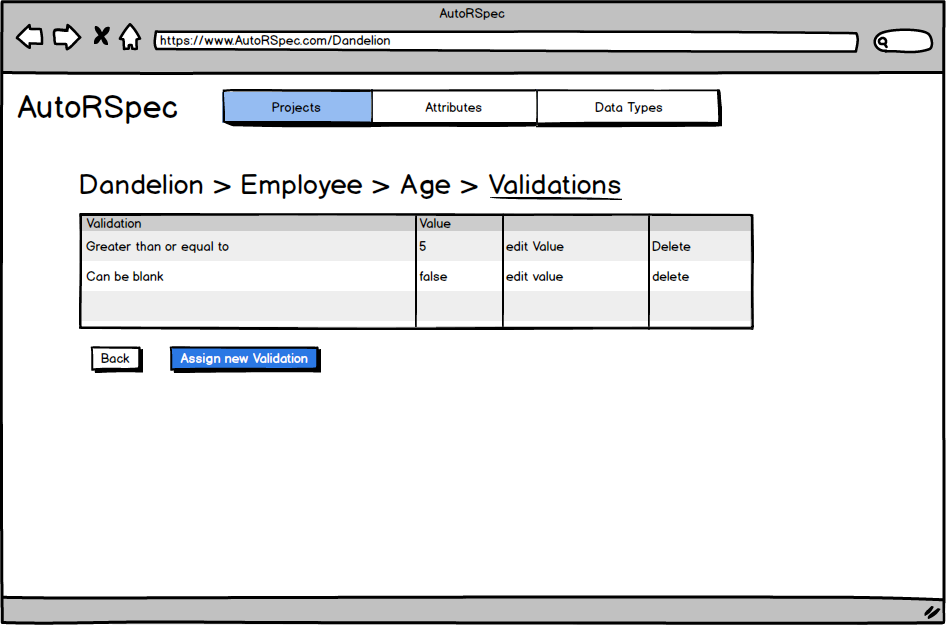
\includegraphics[width=\linewidth]{screenshots/mutable}
\caption{Mock up for a table in the system displaying its fields}
\label{fig:mu2}
\end{figure}

\begin{figure}
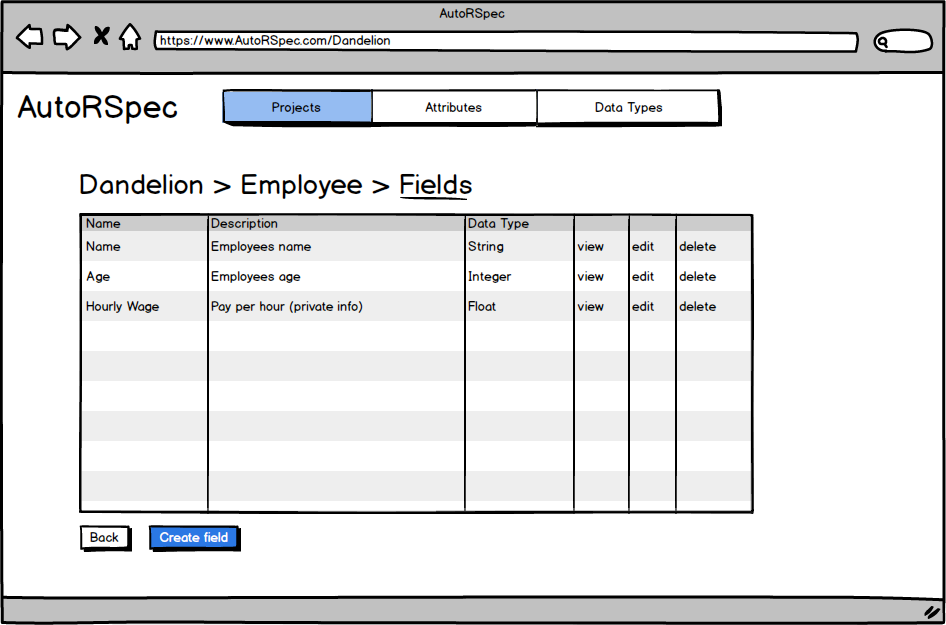
\includegraphics[width=\linewidth]{screenshots/mutablefields}
\caption{Mock up for a field in the system displaying its validation}
\label{fig:mu3}
\end{figure}

\begin{figure}
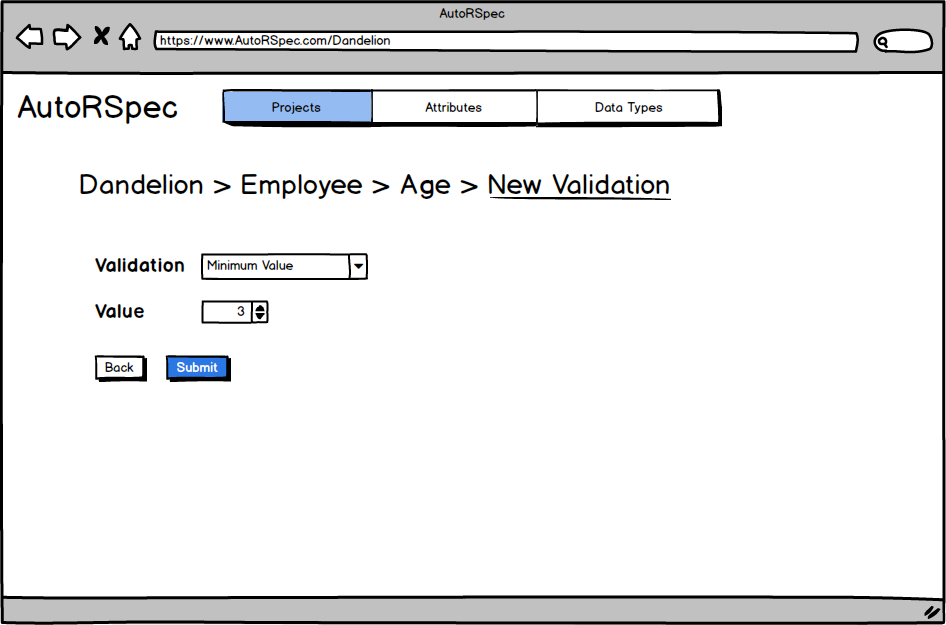
\includegraphics[width=\linewidth]{screenshots/muform}
\caption{Mock up for a form in the system}
\label{fig:mu4}
\end{figure}

\par \textbf{General}
\par Consistiency was at the the forefront of the visual and flow design. Each page that has a dependent entity can only be created via a button on the page of that entity\ref{fig:mu2}. When viewing an entity it will display all and only its dependent entities in a table.\ref{fig:mu2} The dependent entites can be viewed, edited and deleted from this table via links in the row of that entity on the table\ref{fig:mu3}. Each page that is dependent upon on entity can access the dependent enity via the back button\ref{fig:mu3}, also applies naviagtionally to forms\ref{fig:mu4}. The header at the top of each page displays the depth the user is at by underlying the current level while also indicating the levels with the name of the entity at that level\ref{fig:mu3}.

\par \textbf{Nav bar}
\par The nav bar is not a page but the navigational bar displayed at the top of each page\ref{fig:mu1}. It links to the projects page, validations page and the data types page via the appropiatley name button.

\par FUNCTIONALITY OF PAGES ???


\subsection{Test Case Generation}
\subsubsection{Value Generation}
\begin{lstlisting}[frame=single,numbers=left,caption= {Pseudo code for value generation} label={psuedo:value}]
generate_value( (*\textbf{isolatedValidation}*), (*\textbf{validations}*))
 for (*\textbf{iterationCount}*) in (*\textbf{1}*) to (*\textbf{X}*)
  (*\textbf{randomValues}*) = generate_random_values (*\textbf{Y}*)
  if (*\textbf{isolatedValidation} not \textbf{nil}*)
   (*\textbf{randomValues}*) = fail_validation((*\textbf{isolatedValidation}*), (*\textbf{randomValues}*))
   if (*\textbf{randomValues}*) is empty
    next
  for (*\textbf{validation}*) in (*\textbf{validations}*)
   randomValues = pass_validation((*\textbf{validation}*), (*\textbf{randomValues}*))
   if (*\textbf{randomValues}*) is (*\textbf{empty}*)
    (*\textbf{next}*)
  if (*\textbf{randomValues}*) is (*\textbf{empty}*)
   (*\textbf{ next}*)
  else
   (*\textbf{return}*) random value from (*\textbf{randomValues}*)
 return (*\textbf{ERROR NO VALUE GENERATED}*)
\end{lstlisting}

\par The psuedo code in Listing 1 shows then general approach to generating a value for a test case. To increase the efficency and speed of potentailly returning a valid value by generating \textbf{X} values at a time for a potentail of \textbf{Y} times. Generating \textbf{X}*\textbf{Y} values initailly will take a greater deal of time and may be overkill. The correct balance will need to be found in implementation of the initail amount of values for each iteration and how many iterations to carry out.
\par The function will take two parameters, a validation to fail and a list of validations to pass. The validation to fail can be nil, in which case it will produce a value that passes all validations in validations parameter. The validations parameter can also be an empty list in which case it will return a value that fails the isolated validation. In the case of nil validation and and empty list of validations or no value can be generated it will return an error.
\par The flow of the function is to generate a random amount of values, then remove those values that pass the isolated validation, afterwards it will remove those that fail each validation in validations. After each time this array of random values is manipulated it will check if its empty, if so it will skip to the next iteration, this improves speed and efficency by eliminating unnesscary operations. When all validations have been processed it will return a random value from random values. The general flow and principles is the same for each data type that values will be generated.


\subsubsection{RSpec Test Case}
\begin{lstlisting}[frame=single,numbers=left,caption= {Pseudo code for value generation} label={psuedo:case}]
it "is (invalid with a value that is not (*\textbf{VALIDATION}*) (*\textbf{VALVALUE}*)" do
  (*\textbf{TABLENAME}*) = build(:(*\textbf{TABLENAME}*), (*\textbf{FIELDNAME}*): (*\textbf{GENVALUE}*)
  if (*\textbf{TABLENAME}*).respond_to?(:valid?)
   expect((*\textbf{TABLENAME}*).not_to be_valid, lambda (*\textbf{TABLENAME}*).errors.full_messages.join("\\n")
 end
end
\end{lstlisting}

\par \textbf{VALIDATION} is the validation that is being tested on the field, and is described as its polar opposite
\par \textbf{VALVALUE} is the value of the validation that is being tested on the field.
\par \textbf{TABLENAME} is the name of the table the field belongs to
\par \textbf{FIELDNAME} is the name of the field under test
\par \textbf{GENVALUE} is the value that will test the validation
\par The RSpec test case template that will be populated with information from the functional specification and value generated. An example of a employees age field with validation of greater than value eight with a generated value of thirteen.

\begin{lstlisting}[frame=single,numbers=left,caption= {Pseudo code for value generation output} label={psuedo:caseex}]
it "is invalid with a value that is not greater than 8" do
  employee = build(:employee, age: (*\textbf{13}*))
  if employee.respond_to?(:valid?)
   expect(employee.to_not be_valid, lambda employee.errors.full_messages.join("\\n")
 end
end
\end{lstlisting}

\subsubsection{RSpec Test Suite}

\par The test suite is responsible for the overall document structure that the user downloads. It will provide the preamble, then iterate through each field and finally end the document. It will provide all necessary logic to navigate test cases correctly and add the correct syntaxical links to the file. 

\begin{lstlisting}[frame=single,numbers=left,caption= {Pseudo code for value generation} label={psuedo:suite}]
require "spec_helper"

desrcibe "(*\textbf{TABLENAMECAP}*)" do
 it "has a valid factory" do
  expect(build(:(*\textbf{TABLENAME}*))).to be_valid
 end
 #for each field belonging to table |(*\textbf{f}*)|
  describe "(*\textbf{f.NAME}*) has property" do
  # genval = generate_value((*\textbf{nil}*), (*\textbf{f.validations}*))
  # add to file test_case_pass_all((*\textbf{f}*),(*\textbf{genval}*))
  #for each validation belonging to (*\textbf{f}*) |(*\textbf{v}*)|
   # genval = generate_value((*\textbf{v}*), (*\textbf{rest of validations}*))
   # add to file test_case((*\textbf{v}*),(*\textbf{f}*),(*\textbf{genval}*))
  #end
  end
 #end
end
\end{lstlisting}
\par EXAMPLE ??
\par To make the pseudo code more clear lines starting with \# are not printed to the document but code that is ran. TABLENAMECAP is the table name capitalised. Lines 1-4 are the preamble and set up the RSpec document and write a test to check the tables factory is valid. Then for each field it will add the correct syntax to the file for that field and follow it by adding a test case to the file that passes all validations. For each validation that field has been assigned it will iterate through isloting each field and adding the relevant test case to the file. Test suite is the top level function therefor before it calls to generate a test case, lines 8,11, it will call the function to generate a valid value for that test case, lines 7, 10. Test suite will finally end the document with the appropiate "end"  syntax that it opened in the preamble.

\section{Chapter 5: Implemention and Testing}


\subsection{Setup}
\par Ruby version 2.1.7 and rails 4.2.5.2 were used to construct this project.
\par Github\cite{github} was used throughout the project to provide version control and to prevent any catastrophes. The airbnb ruby style convention was used to provide clean looking and consistent code\cite{Airbnb}. Rails new was used to instatiate the system. Then the generate scaffolfd command was used to construct the base for each table in the database schema outlined in chapter 4.1 \ref{fig:scaffold}. This sets up the default mvc components for each, the exact files created can be seen in Figure \ref{fig:scaffold}.

\begin{figure}
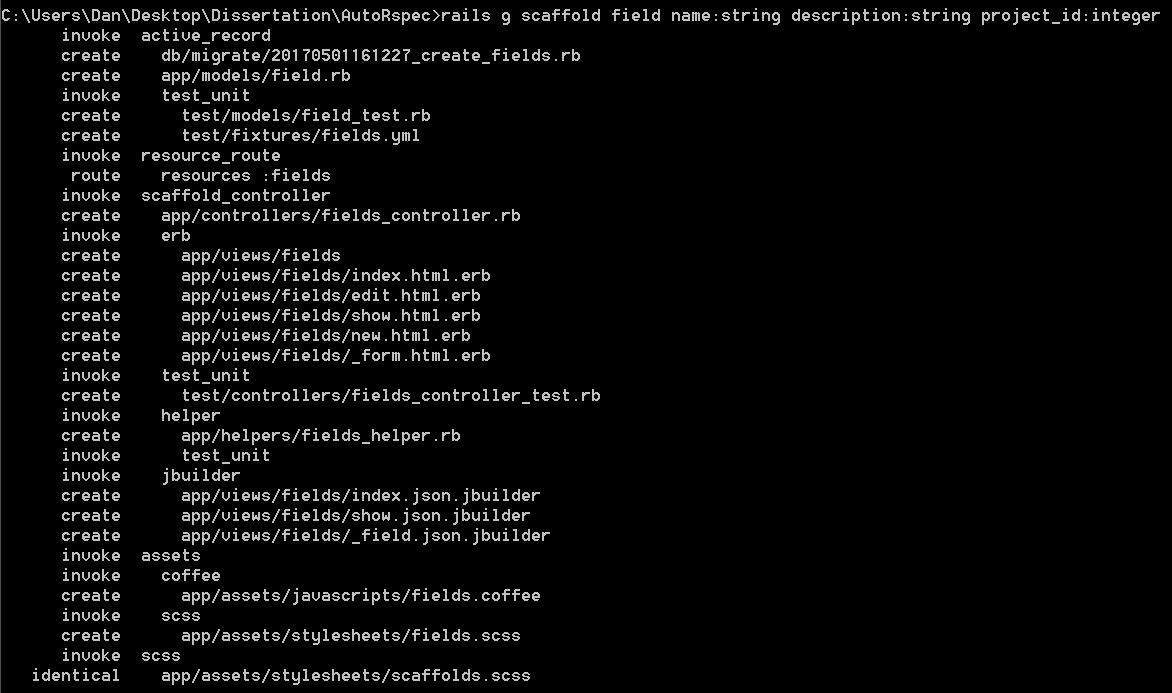
\includegraphics[width=\linewidth]{screenshots/scaffold_example}
\caption{Rails g scaffold command for field}
\label{fig:scaffold}
\end{figure}

\subsection{Database}

\begin{figure}
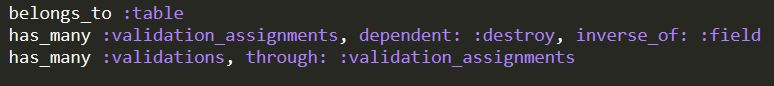
\includegraphics[width=\linewidth]{screenshots/relations}
\caption{Rails native relation methods used in field.rb model}
\label{fig:relations}
\end{figure}

\begin{figure}
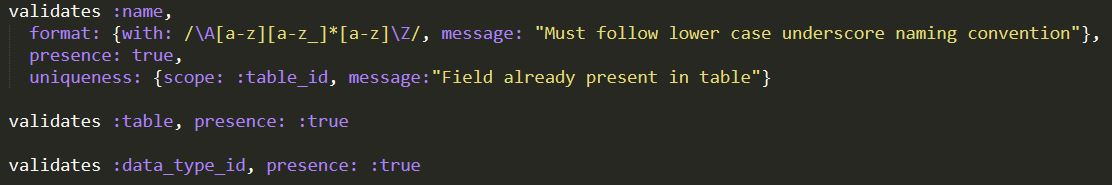
\includegraphics[width=\linewidth]{screenshots/validations}
\caption{Rails native validation method used in field.rb models}
\label{fig:validations}
\end{figure}

\subsection{View and Flow}


\subsection{Test Case Generation}


\subsubsection{Value Generation}


\subsubsection{RSpec Test Case}


\subsubsection{RSpec Test Suite}



\section{Chapter 6: Results and Discussion}
Filler text, filler text, filler text, filler text, filler text, filler text, filler text, filler text.
\section{Chapter 7: Conclusions IGNORE THIS CHAPTER, GRAVEYARD}

\par Software disasters can be caused by poor testing practices,\cite{mcquaid2012software} if the correct testing procedures practices were in place the situation would never of occured. Software testing is therefore extremely important and included in the development of all applications. However software testing "In a typical programming project approximately 50 percent of the elapsed time and more than 50 percent of the total cost were expended in testing the program or system being developed"\cite{myers2011art}, making it a huge cost of development. By automating part or the whole of the process the costs can be reduced while still obtaining all of the benefits.

\subsection{Benefits of Testing and Automation}

\par Inadequate software testing infastructure was estimated to cost the US economy \$59.5 billion a year.\cite{NISTReport} It was also estimated that the potentail cost reduction from feasbile infastructure would be \$22.2 billion a year. \cite{NISTReport} Due to software disasters and the vast amount of money that can be saved and also avoid incurring additonal costs, people have become more aware of the importance of testing. The benefits of the reduced costs  comes from ihe increased reliabilty and quality of the product produced when software testing is implemented.

\par "In a typical programming project approximately 50 percent of the elapsed time and more than 50 percent of the total cost were expended in testing the program or system being developed"\cite{myers2011art}. Software testing saves you alot of money but also costs alot of money. By automating part or the whole process the costs can be reduced while still obtaining all of the benefits.



\subsection{Ruby on Rails}
\par Ruby on Rails as a framework 
\par model as mvc
\par Rspec to test m

\subsection{Project Aims}
\par The overall aim of this project is to reduce the cost of developing Ruby on Rails applications. The reduction in costs comes from the time saved by automatically generating test cases for the model component of the application. The develop will input a formal specification of thier database into a system from which they can download seperate files containing a test suite for each table they have defined. The files are seperated in keeping with standard Ruby on Rails practices. Once the file is downloaded it can be inserted into the application and be available to run immediatley. This project should reduce the errors and bugs in Ruby on Rails applications via the feedback from the tests generated, improving the reliablity and quality of Ruby on Rails projects via the model component.

\par The derivation of information makes the test more focused on the actual implementation of the code rather than its specified behaviour. Test cases tend to be at a much finer grain than black box testing individual methods. Tests are designed to execute a particular behaviour within the program, such as testing how it handles a binary overflow.\cite{nidhra2012blackbox}\cite{young2008software}
\subsection{Project Limitations}

\par Rails and its do more with less, inline with automated testing..

\par The aims of the project are to:
\begin{enumerate}
\item Reduce the amount of time it takes for a User to produce tests for model validation
\item Produce tests that are of high readable quality
\item Produce tests that fully test properties specified
\item The process should be hassle free
\end{enumerate}

\par Challenges that the project faces are
\begin{enumerate}
\item Identifying the minimum information required to produce tests
\item Creating a process that is hassle free
\item Natural language in tests that is appears human written
\item Generating the tests in an acceptable time frame
\item Building an efficent database structure for the information
\end{enumerate}

Filler text, filler text, filler text, filler text, filler text, filler text, filler text, filler text.
Hello World!
\subsection{subsection}
Structuring a document is easy!! \cite{near2012rubicon}
\subsubsection{subsubsection}
\paragraph{p1}
It's a me, Mario\footnote{\label{myfootnote}\cite{near2012rubicon}}.
\subparagraph{sp1}
Wwoohooo
\section{image}
\begin{figure}
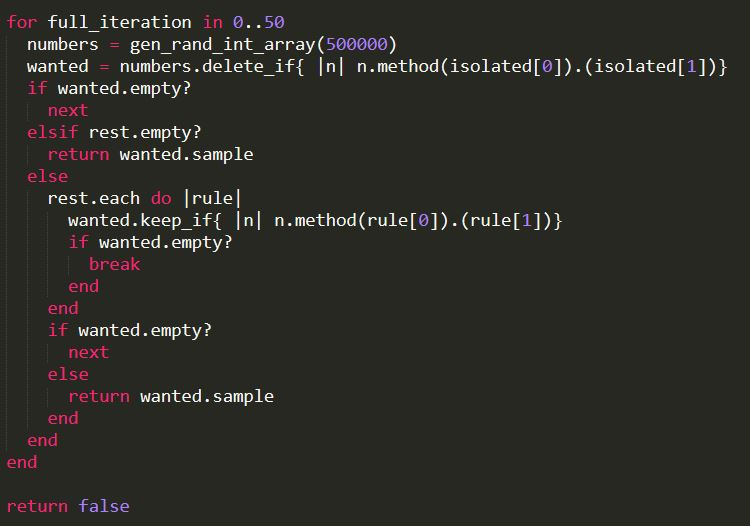
\includegraphics[width=\linewidth]{screenshots/code-gen-int-pre_divisible_keep_if}
\caption{caption for image, shown below image}
\label{fig:code1}
\end{figure}
Figure \ref{fig:code1} shows some savage code

	
\begin{table}[h!]
\centering
\caption{Caption for the table.}
\label{tab:table1}
\begin{tabular}{ccc}
\toprule
Some & actual & content\\
\midrule
prettifies & the & content\\
as & well & as\\
using & the & booktabs package\\
\bottomrule
\end{tabular}
\end{table}

\begin{table}
\caption{Data Types Supported}
\label{tab:datatypessupported}
    \begin{tabular}{|l|}
        \hline
        Data Type \\ \hline
        Integer   \\ 
        Float     \\ 
        String    \\
        \hline
    \end{tabular}
\end{table}

\begin{table}
\caption{Integer and Float Validations Supported}
\label{tab:integersupported}
    \begin{tabular}{|l|}
        \hline
        Validation               \\ \hline
        Blank                    \\ 
        Inclusion                \\ 
        Exclusion                \\ 
        Greater Than             \\ 
        Greater Than or Equal To \\ 
        Equal To                 \\ 
        Less Than or Equal To    \\ 
        Less Than                \\ 
        Other Than               \\ 
        Divisible                \\
        \hline
    \end{tabular}
\end{table}

\begin{table}
\caption{String Validation Supported}
\label{tab:stringsupported}
    \begin{tabular}{|l|}
        \hline
        Validation     \\ \hline
        Blank          \\ 
        Inclusion      \\ 
        Exclusion      \\ 
        Minimum Length \\ 
        Maximum Length \\ 
        Exact Length   \\ 
        Format         \\
        \hline
    \end{tabular}
\end{table}


\bibliography{bibliography}
\bibliographystyle{ieeetr}
\end{document}
